\documentclass[dvipdfmx,11pt,a4paper,oneside,openany]{jsbook}
\usepackage{package}
%\usepackage{a4wide}
\usepackage[dvipdfmx]{hyperref}
\usepackage{pxjahyper}


%\title{}
%\author{}
%\date{\today}
\begin{document}
%\maketitle

%\tableofcontents

%\makeatletter
%\@addtoreset{equation}{section}
%\def\theequation{\thesection.\arabic{equation}}
%\makeatother
\newcommand{\ctext}[1]{\raise0.2ex\hbox{\textcircled{\scriptsize{#1}}}}

\addtolength{\fullwidth}{-26truemm} %全体の幅(ヘッダ部の幅)を既定値から26mm小さくする
\setlength{\textwidth}{\fullwidth}  %本文の幅(textwidth)を全体の幅(=ヘッダ部の幅)にそろえる
\setlength{\evensidemargin}{10truemm}   %偶数ページの左余白を10mm(+1インチ)にする
\setlength{\oddsidemargin}{10truemm}    %奇数ページの左余白を10mm(+1インチ)にする
\chapter{Preface cum introduction}
\begin{itembox}[l]{目的}
    非線形方程式の古典解のうち,ミンコフスキー計量やユークリッド方程式における場の方程式に対応するものがいくつかあり,そういった古典解から相対論的量子場の理論の情報を得る.
\end{itembox}
本ゼミにおいてのメインテーマとなるソリトンとインスタントンであるが,どちらも簡単にいえば形状を保ったまま進行し互いに衝突しても崩れないような局在化(localized)した波の事である.そもそもソリトンの英語スペルはsolitonであり,これはsolitary(孤立した)+on(粒子につける接尾辞(Fermi{\bf on}, Bos{\bf on}, Glu{\bf on}, Phot{\bf on} \dots))から来ている.すなわち孤立した波の塊でありながら歪むことなく安定に一様な速度で進行する波であり,粒子的に振る舞うような物理的対象を指す.ここで,なぜ局在化した波が粒子としてみなせるかということについては場の理論において場が作る波をエネルギーのたまり場のようなものであると捉えると,ポツンと局在化したエネルギーが非離散的(連続的)に形を崩さずに移動していればまるで粒子が移動していると拡大解釈できることから理解できる.

このようなソリトンは様々な応用が効く.本来素粒子は量子論で語られるべきものであるが,相対論的な場の理論から素粒子もlocalizeされたエネルギーパケットをもっていることがわかっており,古典場の理論からスタートするソリトンを用いてその振る舞いを説明することができ,ソリトンが古典論と量子論をつなげる可能性を持ち合わせていることを意味する.他にもソリトンには原子核,陽子中性子の模型や宇宙論のテクスチャ,物性の磁気スカーミオンなど素粒子原子核から物性,宇宙まで様々な分野において重要な役割を果たす.

\begin{figure}[H]
    \centering
    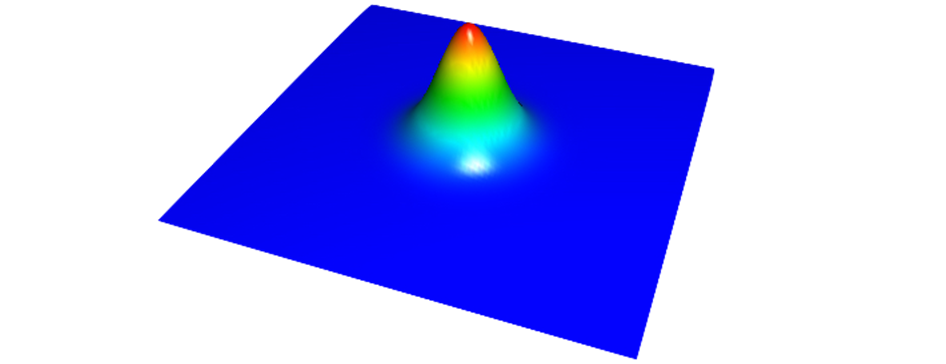
\includegraphics[width=4cm]{figure/soliton.png}
    \caption{ソリトン}
    \label{soliton}
\end{figure}

\chapter{CLASSICAL SOLITONS AND SOLITARY WAVES}
\section{Introduction}
本章におけるメインテーマはsin-Gordons solitonやkinkの$\phi^4$理論や'tHooft-Polyakov monopoleやインスタントンなどの例を用いながらソリトン(Solitons)と孤立波(Solitary waves)の区別をつけるということである.

また,以下にこれから使う記法についてまとめておく.
\begin{screen}
    \begin{itemize}
        \item 空間と時空の座標系はベクトル$x^{\mu}(\mu=0, 1, 2, 3, ; x^{0}\equiv ct, x^{1}=x, x^{2}=y, x^{3}=z)$で与えられる.
        \item 上付きまたは下付きの添字はミンコフスキー計量テンソル$g_{\mu \nu}=g^{\mu \nu}$;
              \begin{align*}
                  g_{\mu \nu}=
                  \left(\begin{array}{cccc}
                          1 & 0  & 0  & 0  \\
                          0 & -1 & 0  & 0  \\
                          0 & 0  & -1 & 0  \\
                          0 & 0  & 0  & -1
                      \end{array}\right)
              \end{align*}
              で書かれる.(Mostly minus)
        \item 同じ添字がついてるものについては足し上げる.(縮約記法)
        \item $\partial_{\mu}$は時間や空間での微分$\frac{\partial}{\partial_{\mu}}$を表す.
        \item 簡単のために本セクションに限っては1つの時間座標と1つの空間座標の(1+1)次元,つまり$\mu=0,1$とする.
    \end{itemize}
\end{screen}

\section{Solitary waves and solitons}
先に述べたようにSolitonとSolitary waveは非線形の波動方程式においてどちらも局在化した特別な特徴をもつ解でありその区別がどのようにできるかを学ぶ.

\subsection{Case of the simplest wave equation}
まず,よくある最もシンプルな線形かつ非分散的である波動方程式
\begin{align}
    \Box\phi & =\partial^{\mu}\partial_{\mu}\phi\nonumber                                                                             \\
             & =\left(\dfrac{1}{c^2}\dfrac{\partial^2}{\partial t^2}-\dfrac{\partial^2}{\partial x^2}\right)\phi(x,t)=0\label{eq:2.1}
\end{align}
を考える.この解は以下のような2つの特徴をもつ.
\begin{description}
    \item[(i)] 解である$f(x\pm ct)$は全領域で一意に定まり,微分が定義され,連続である(well-behaved function).また,$\omega=kc$とすれば$\cos(kx\pm \omega t)$と$\sin(kx\pm \omega t)$の平面波はどちらも式(\ref{eq:2.1})の1つの解となっておりフーリエ変換で重ね合わせれば
          \begin{align}
              f(x-c t)=\int \mathrm{d} k\left[a_{1}(k) \cos (k x-\omega t)+a_{2}(k) \sin (k x-\omega t)\right]
          \end{align}
          とかける.そして仮に局在化した解$f(x-ct)$をもってきた場合,その波のパケットは一定速度$\pm c$で歪みや形の崩れなく進む.
    \item[(ii)] 波動方程式が線形であるが故に解として波のパケット$f_1(x-ct)$と$f_2(x+ct)$が与えられれば,それらの線形結合である
          \begin{align*}
              f_3(x,t)=f_1(x-ct)+f_2(x+ct)
          \end{align*}
          もまた解となる.

          そして$t\rightarrow-\infty$で$f(x,t)$は2つのパケットをそれぞれ別の方向に向かって二分し,その後時間をかけて互いに歪まずに接近し衝突する.そして衝突後も形を崩さず$t\rightarrow\infty$に向かって同じ2つのパケットが一定の速度で移動していく.
\end{description}
つまりこれらを簡単にまとめれば式(\ref{eq:2.1})の解は以下の性質を持つ.
\begin{screen}
    \begin{description}
        \item[(i)] 1つのパケットが歪まず,形を維持したまま一定速度で移動する.
        \item[(ii)] いくつかのパケットが互いに衝突したとしてもその進行速度と形が維持される.(別ファイルに添付したGifを参照.)
    \end{description}
\end{screen}
\begin{figure}[H]
    \centering
    \subfigure[]{%
        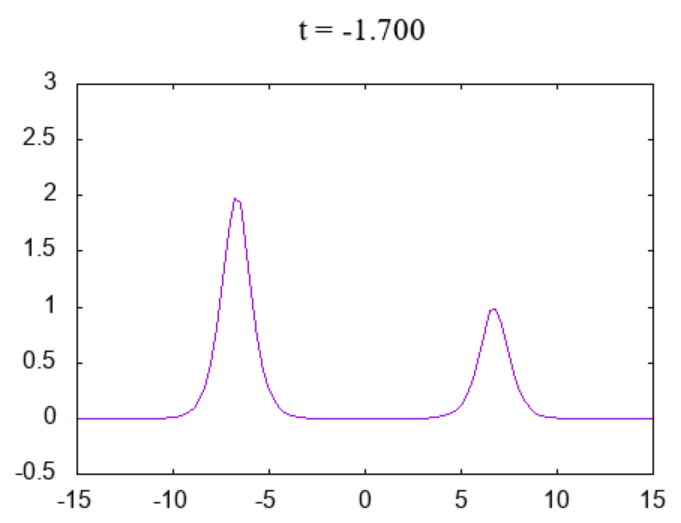
\includegraphics[clip, width=0.4\columnwidth]{figure/2-soliton1.png}}%
    \subfigure[]{%
        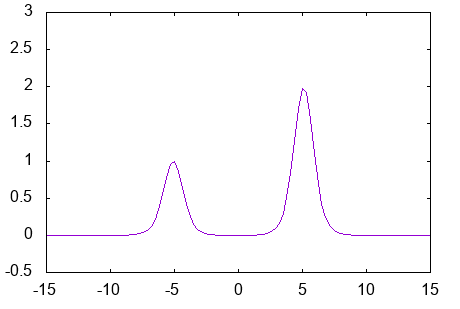
\includegraphics[clip, width=0.4\columnwidth]{figure/2-soliton2.png}}%
    \label{2-soliton}
\end{figure}

\subsection{Case of Klein-Gordon equation}
しかしながら大半の波動方程式は非線形項を含んでいたり,分散的であったりと複雑で全ての波動方程式が性質(i),(ii)を満たしているとは限らない.

そのうちの一つが式(\ref{eq:2.1})に$m^2c^2$の項を加えたKlein-Gordon方程式
\begin{align}
    \left(\square+m^{2} c^{2}\right) \phi(x, t) & \equiv\left(\frac{1}{c^{2}} \frac{\partial^{2}}{\partial t^{2}}-\frac{\partial^{2}}{\partial x^{2}}+m^{2} c^{2}\right) \phi(x, t)\nonumber \\
                                                & =0
\end{align}
がある.これは明らかに先と同様に線形であり,かつ$\cos(kx\pm \omega t)$と$\sin(kx\pm \omega t)$の平面波解をもつ.しかし今回の場合は$\omega^2=k^2c^2+m^2c^4$であり分散的という違いがある.いま先と同様に線形であることを用いて局在化したパケット解
\begin{align*}
    f(x-ct)=\int \mathrm{d} k\left[a_{1}(k) \cos (k x-\omega t)+a_{2}(k) \sin (k x-\omega t)\right]
\end{align*}
を作ったときに今回の場合,波の進行速度が$\omega(k)/k$というように波数$k$に依存することになる.したがって一度作った波のパケットが時間とともに違った速度で形を広げながら伝搬してしまい,先に述べた(i)(ii)の特徴を持ち合わせていないということがわかる.(別ファイルに添付したGifを参照.)
\begin{figure}[H]
    \centering
    \subfigure[]{%
        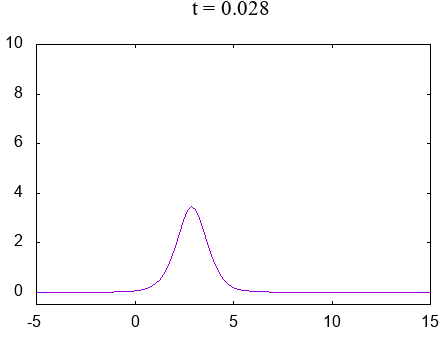
\includegraphics[clip, width=0.53\columnwidth]{figure/wave(spread)1.png}}%
    \subfigure[]{%
        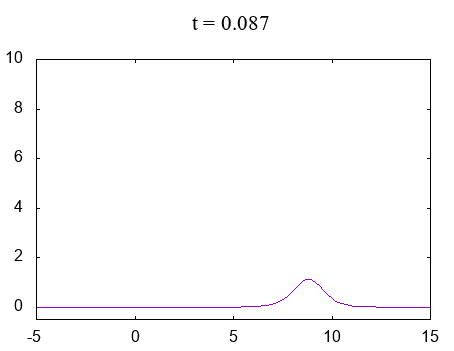
\includegraphics[clip, width=0.55\columnwidth]{figure/wave(spread)2.png}}%
    \label{wave(spread)}
\end{figure}
なお紹介だけにはなるが,他には解析的には解けないが式(\ref{eq:2.1})に$\phi^3$の項を付け加えたような以下の非線形波動方程式も(i)(ii)の特徴を持ち合わせていない.
\begin{align}
    \left(\frac{1}{c^{2}} \frac{\partial^{2}}{\partial t^{2}}-\frac{\partial^{2}}{\partial x^{2}}\right) \phi(x, t)+\phi^{3}(x, t)=0\label{eq:2.4}
\end{align}

\subsection{View of energy density}
先の議論を踏まえて一般的にはSolitonとSolitary-waveの以下のような区別がなされている.
\begin{screen}
    \begin{itemize}
        \item (i)の特徴を満たすもの $\cdots$ {\bf Solitary-wave}, {\bf Soliton}
        \item (i)を及び(ii)の特徴を満たすもの $\cdots$ {\bf Soliton}
    \end{itemize}
\end{screen}

しかしこれではどういったときに(i)または(ii)の特徴を満たすのかはわかっておらず,普遍的ではない.

ここで場$\phi_i$の波自体に着目するのではなく,むしろ場$\phi_i$がつくるエネルギー密度$\epsilon$に着目してみる.まず条件としては以下のような設定を課す.
\begin{itemize}
    \item 空間内の全エネルギー$E[\phi_i]$は保存し,一般性を失わない.
    \item エネルギー$E$の最小値は0.
    \item 空間内でエネルギーは有限の値をとるが無限遠では$E=0$.
    \item 任意の時刻$t$において十分遠方($x\rightarrow \infty$)で最小値$E[\phi_i]$に漸近するような場の方程式の解に対して局在化した(localized)という言葉をつかう.
\end{itemize}
ではこれらをいくつかの例を紹介しながらlocalizeするとはどういうことか見ていく.先に紹介した式(\ref{eq:2.4})の方程式
\begin{align*}
    \left(\frac{1}{c^{2}} \frac{\partial^{2}}{\partial t^{2}}-\frac{\partial^{2}}{\partial x^{2}}\right) \phi(x, t)+\phi^{3}(x, t)=0
\end{align*}
においては場$\phi$が作るエネルギーを見てみると
\begin{align}
    E[\phi]=\int_{-\infty}^{\infty} \mathrm{d} x\left[\frac{1}{2 c^{2}}\left(\frac{\partial \phi}{\partial t}\right)^{2}+\frac{1}{2}\left(\frac{\partial \phi}{\partial x}\right)^{2}+\frac{1}{4} \phi^{4}\right]
\end{align}
で与えられる.これは$\phi=0$で最小値$E[\phi]$をとるから,localizeすると言いたければ,十分遠方$x\rightarrow \infty$で$\phi(x,t)\rightarrow 0$となっていれば良い.\\

他には自発的対称性の破れを記述する有名な
\begin{align}
    \frac{1}{c^{2}} \frac{\partial^{2} \phi}{\partial t^{2}}-\frac{\partial^{2} \phi}{\partial x^{2}}-\phi+\phi^{3}=0
\end{align}
という非線波動方程式におけるエネルギーは
\begin{align}
    E[\phi]=\int_{-x}^{x} \mathrm{d} x\left[\frac{1}{2 c^{2}}\left(\frac{\partial \phi}{\partial t}\right)^{2}+\frac{1}{2}\left(\frac{\partial \phi}{\partial x}\right)^{2}+\frac{1}{4}\left(\phi^{2}-1\right)^{2}\right]
\end{align}
で与えられる.この$E[\phi]$は$\phi(x,t)=\pm 1$で最小値をとるから,localizeすると言いたければ,十分遠方$x\rightarrow \pm\infty$で$\phi(x,t)\rightarrow \pm 1$となる必要がある.

\subsubsection{Solitary wave}
localizeするとはどういうことかが普遍的に述べられた上でエネルギー密度の観点からSolitary waveとは何かを考える.Solitary waveは場の方程式においてlocalizeしているという特異性だけでなく次のような時空依存のエネルギー密度を描くものと定義できる.
\begin{align}
    \epsilon(\bm{x},t)=\epsilon(\bm{x}-\bm{u}t)\quad (\bm{u}: \text{速度ベクトル})\label{eq:2.8}
\end{align}
これは明らかに場が作るエネルギー密度のパケットが一定の速度で形が変わらずに移動するという(i)の特徴を表現できており,これがまさにSolitary  waveの定義とできる.

\subsubsection{Soliton}
次にSolitonについてもエネルギー密度の観点からその定義を考える.Solitonは先の議論の特徴(i)だけでなく特徴(ii)に重きを置く必要がある.特徴(ii)はいくつかのパケットが互いに衝突したとしてもその進行速度と形が維持されるということであった.そこで以下のような状況設定で議論を進める.
\begin{itemize}
    \item 非線形波動方程式でlocalizeした$N$個のsolitary wave解$\epsilon_0(\bm{x}-\bm{u}t)$で解が構成されている.
\end{itemize}
上記の状況を式で表せば
\begin{align}
     & \varepsilon(\bm{x}, t) \rightarrow \sum_{i=1}^{N} \varepsilon_{0}\left(\bm{x}-\bm{a}_{i}-\bm{u}_{i} t\right), \quad \text { as } t \rightarrow-\infty\label{eq:2.9}                  \\
     & \varepsilon(\bm{x}, t) \rightarrow \sum_{i=1}^{N} \varepsilon_{0}\left(\bm{x}-\bm{a}_{i}-\bm{u}_{i} t+\bm{\delta}_{i}\right), \quad \text { as } t \rightarrow+\infty\label{eq:2.10} \\
     & \qquad \ \ \ \ \ \ \ \ \ \ \ \ \ \ \ \ \ \ \ \ \  \ \ \ \ \ \ \ \ \ \ \ \ \ \ \ \ (\bm{a}_i,\bm{\delta}_i:\text{定ベクトル})\nonumber
\end{align}
となる.これは$t\rightarrow -\infty$であるいくつかのSolitary waveのエネルギーパケットをもった解が一定速度かつ歪みなく進んだのち$t\rightarrow \infty$で時間発展したとしても形が変わらないという特徴(ii)の描像を描けているといえる.つまりこのエネルギー密度の関係式を満たすものがSolitonであると定義できる.\\

以上でSolitonとSolitary waveの区別ができるようになった.そしてこの世界には静的解を含めてSolitary waveは割と存在する.しかしながらSolitonは式(\ref{eq:2.10})の要請の縛りが強くほとんど存在しないというのが現状である.そもそも非線形場の方程式に対してSolitary waveの要請式(\ref{eq:2.8})を確認するのも割と大変な作業となる.そして式(\ref{eq:2.9})(\ref{eq:2.10})の両方を満たしているかを確認するのはさらに労力が必要となる.(この本ではやりたきゃ一人で時間をかけてやってどうぞと記載してある.)また,物理でSolitonと使われるとき大体はSolitary waveも含めてそう呼ぶ慣習があり,重要なことはその違いを理解していることである.研究等なんらかの場合に厳密にSolitonであることを示す必要がある場合には式(\ref{eq:2.8})(\ref{eq:2.9})(\ref{eq:2.10})の要請を確かめられれば良い.一応逆散乱法やバックグラウンド変換などといったエレガントな方法も存在するということも紹介しておく.

\section{Some solitary waves in two dimensions}
\subsection{Static Solitary wave and boundary conditions}
解が時間依存していない静的解もSolitary waveであったからそのいくつか簡単な例について2次元系で見ていく.

以下のようなローレンツ不変なラグランジアン密度
\begin{align}
    \mathscr{L}(x, t)=\frac{1}{2}(\dot{\phi})^{2}-\frac{1}{2}\left(\phi^{'}\right)^{2}-U(\phi)
\end{align}
を考える.\footnote{プライム記号("$'$")は時間微分を表しドット記号("$\dot{ }$")は空間微分を表す.}なおここでは光速$c=1$とし,ポテンシャル$U(\phi)$は$\phi$の関数で最小値が0のものとする.作用の変分をとれば
\begin{align}
    \delta\left(\int dt \int_{-x}^{x}dx\mathscr{L}(x,t)\right)=0
\end{align}
となりこの内の一つから以下の波動方程式が導かれる.
\begin{align}
    \square \phi \equiv \ddot{\phi}-\phi^{''}=-\frac{\partial U}{\partial \phi}(x, t)\label{eq:2.13}
\end{align}
そしてエネルギーの関数は
\begin{align}
    E[\phi]=\int_{-\infty}^{\infty} \mathrm{d} x\left[\frac{1}{2}(\dot{\phi})^{2}+\frac{1}{2}\left(\phi^{'}\right)^{2}+U(\phi)\right]\label{eq:2.14}
\end{align}
となる.(求め方はAppendixにまとめた.)そして$U(\phi)$が$M(\geq1)$個の点で最小値0をとする.
\begin{align}
    U(\phi)=0 \quad \text { for } \quad \phi=g^{(i)} ; \quad i=1, \ldots, M\label{eq:2.15}
\end{align}
また,仮に場$\phi(x,t)$が定数であれば式(\ref{eq:2.14})のエネルギーも最小値$E[\phi]=0$を
\begin{align}
    \phi=g^{(i)} ; \quad i=1, \ldots, M
\end{align}
でとる.

いま我々は簡単のために静的解のSolitary waveを考えるから式(\ref{eq:2.14})において時間の項を消せば
\begin{align}
    \phi^{''}(x) \equiv \frac{\partial^{2} \phi}{\partial x^{2}}=+\frac{\partial U}{\partial \phi}(x)\label{eq:2.17}
\end{align}
となる.

さらにSolitary waveは有限のエネルギーでlocalizeしたエネルギー密度をもっているという要請をこれに課す.前セクションで述べたが,localizeするには任意の時刻$t$において十分遠方($x\rightarrow \pm\infty$)で最小値$E[\phi_i]$に漸近する必要があった.(($\partial\phi/\partial x\rightarrow 0$も.))いま式(\ref{eq:2.15})で最小値をとることがわかっているから,localizeするという要請から以下の境界条件が成立する.
\begin{screen}
    \begin{align*}
        U(\phi)\rightarrow0 \quad \text{and} \quad \left(\frac{\partial\phi}{\partial x}\right)\rightarrow 0,\qquad \text{as}\quad x\rightarrow \pm \infty
    \end{align*}
\end{screen}

\subsection{Solve the equation (\ref{eq:2.17})}
式(\ref{eq:2.17})をよく見ればニュートンの第二法則と同じになっていることに気付く.というのも$x\rightarrow t$,場$\phi$を質点(analogue particle)の位置座標と捉えればこれは単なるポテンシャルが$-U(\phi)$の運動方程式である.このことからこの運動の全エネルギーは
\begin{align}
    W \equiv \frac{1}{2}\left(\frac{\mathrm{d} \phi}{\mathrm{d}x}\right)^{2}-U(\phi)\label{eq:2.18}
\end{align}
となることがわかる.ここで先に述べた境界条件を課せば$W=0$のゼロエネルギーとなる.また式(\ref{eq:2.14})で与えられる実際の系においてのエネルギーに立ち返ってみても
\begin{align}
    E=\int_{-\infty}^{\infty}\left[\frac{1}{2}\left(\frac{\mathrm{d}\phi}{\mathrm{d}x}\right)^2+U(\phi)\right]\mathrm{d}x
\end{align}
となり,これは明らかにanalogue粒子の運動の作用積分と同じ形になっていることがわかる.したがって,この静的解は粒子のゼロエネルギー($W=0$)の軌道の有限作用に対応しているといえる.

さらに式(\ref{eq:2.17})を解いてみる.両辺に$\phi'$をかけて積分すれば
\begin{align}
    \phi'\phi''=\frac{\partial U}{\partial\phi}\nonumber                                            \\
    \Rightarrow \int\phi'\phi''\mathrm{d}x=\int\frac{\partial U}{\partial \phi}\mathrm{d}x\nonumber \\
    \Rightarrow \frac{1}{2}\left(\phi'\right)^2=U(\phi)\label{eq:2.20}
\end{align}
となる.(なおここで境界条件である$x\rightarrow \pm \infty$で$U(\phi)\rightarrow 0, (\partial \phi/\partial x)\rightarrow 0$を課すことで積分定数はゼロと定まっている.)式(\ref{eq:2.20})はまさにanalogue粒子におけるビリアル定理に対応していることがみてとれる.

\subsection{Some potential}
\subsubsection{Case of potential which have unique minimum}
先の結果を踏まえていくつかのポテンシャル上でanalogue粒子がどのような振る舞いをするかをみてみる.まず図\ref{potential1}のような$\phi=\phi_1$で最大値$U(\phi_1)=0$を取るようなポテンシャルを考える.このときanalogue粒子のゼロエネルギーの軌道はポテンシャル上で$\phi=\phi_1$で最大値0をとりその他は常に負の値をとる.ここでSolitary waveの境界条件に立ち返ってみると,十分遠方($x\rightarrow \pm \infty$)で$\phi=\phi_1$となる必要があるが,図を見てもわかるように例えば$x\rightarrow -\infty$で$\phi=\phi_1$だった場合に$x\rightarrow \infty$で$\phi=\phi_1$にもう一度なることは決してできない.というのも式(\ref{eq:2.18})において$W=0$であったから,仮に$\phi=\phi_1$から右か左のどちらかに転がっていってしまった場合常に$[-U()\phi)]$は負の値で小さくなっていくから$W=0$に保つために運動エネルギー項($1/2(\mathrm{d}\phi/\mathrm{dx})^2$)は常に正で値が大きくなる.つまり一度$\phi=\phi_1$から進んだら粒子は止まることができなくなる.つまりこのポテンシャルでは解かずしてSolitary waveにはなり得ないということがわかる.

\begin{figure}[H]
    \centering
    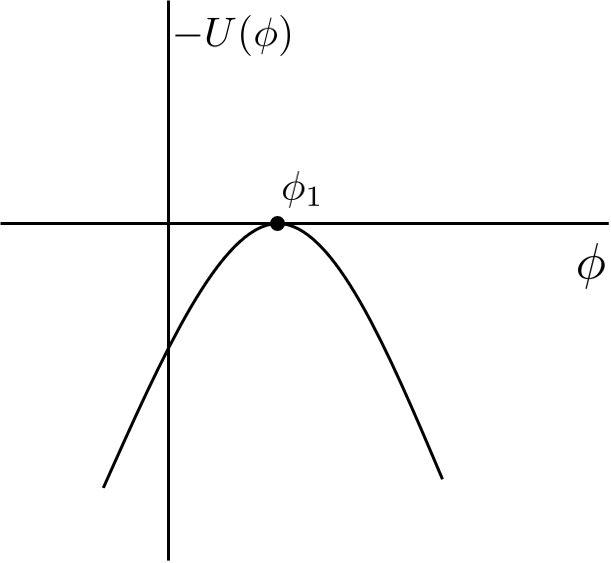
\includegraphics[width=5cm]{figure/potential1.png}
    \caption{(a)}
    \label{potential1}
\end{figure}

\subsubsection{Case of potential which have degenerate minima}
次に2個以上最小値が存在する例として図\ref{potential2}のようなポテンシャルを考える.このポテンシャルは$\phi=\phi_1,\phi_2,\phi_3$の3つの場所で最小値をとる.境界条件を満たすには$x\rightarrow \pm \infty$で$\phi$が3つの値のどれかになる必要があるが,今回の場合それが可能である.考えうるパターンとしては以下の4つに限られる.
\begin{enumerate}
    \item $x\rightarrow -\infty$で$\phi=\phi_1$をスタートし,$x\rightarrow \infty$で$\phi=\phi_2$となる.
    \item 1.の進行方向が逆パターン.
    \item $x\rightarrow -\infty$で$\phi=\phi_2$をスタートし,$x\rightarrow \infty$で$\phi=\phi_3$となる.
    \item 3.の進行方向が逆パターン.
\end{enumerate}
これは$x\rightarrow -\infty$で$\phi_1$にスタートし,$x\rightarrow \infty$で$\phi_2$に至る場合を例にして考えると境界条件から$\phi_2$に至ったときには$U(\phi)$と$\mathrm{d}U/\mathrm{d}\phi$はゼロとなっていることに起因する.式(\ref{eq:2.20})及び式(\ref{eq:2.17})において$\phi'$の速度や加速度などは全て
\begin{align}
    \phi^{'''}=\frac{d}{\mathrm{d} x}\left(\frac{\mathrm{d} U(\phi)}{\mathrm{d} \phi}\right)=\frac{\mathrm{d}^{2} U}{\mathrm{d} \phi^{2}} \phi^{'}=0\nonumber \\
    \phi^{''''}=\frac{\mathrm{d}^{2} U}{\mathrm{d} \phi^{2}} \phi^{''}+\frac{\mathrm{d}^{3} U}{\mathrm{d} \phi^{3}}\left(\phi^{'}\right)^{2}=0 \text { etc. }
\end{align}
というようにゼロになって消えてしまう.したがって$\phi_2$を超えて$\phi_3$に進んだり,$\phi_1$に再び戻ったりというパターンは完全になくなり,上記の4パターンに限られる.そしてこの4パターンでのみSolitary waveが存在しうるということになる.

\begin{figure}[H]
    \centering
    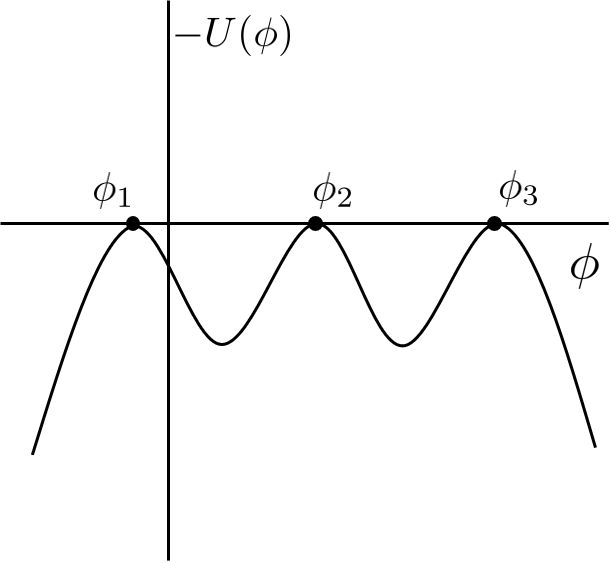
\includegraphics[width=5cm]{figure/potential2.png}
    \caption{(b)}
    \label{potential2}
\end{figure}

以上2つのポテンシャルの例から一般的に以下のようなことが言える.
\begin{screen}
    \begin{description}
        \item[(i)] $U(\phi)$の最小値が1つの場合,静的なSolitary waveは存在しない.
        \item[(ii)] $U(\phi)$が$n$個の最小値を保つ場合,静的なSolitary waveは$2(n-1)$個存在する.
    \end{description}
\end{screen}

\subsection{Solve the equation (\ref{eq:2.20}) with specific potential}
式(\ref{eq:2.20})を実際にポテンシャルを当てはめて解いてみる.
\begin{align}
    \frac{1}{2}(\phi')^2=U(\phi)\nonumber                                                        \\
    \Rightarrow \frac{\mathrm{d}\phi}{\mathrm{d}x}=\pm\left[2U(\phi)\right]^{1/2}\label{eq:2.22} \\
    \Rightarrow x-x_0=\pm\int_{\phi(x_0)}^{\phi(x)}\dfrac{d\bar{\phi}}{[2U(\bar{\phi})]^{1/2}}\label{eq:2.23}
\end{align}


\subsubsection{Case of static solution}
まず静的解の場合について求めるために'kink'と呼ばれる以下のラグランジアン密度を考える.
\begin{align}
    \mathscr{L}(x, t)=\frac{1}{2}\left(\frac{\partial \phi}{\partial t}\right)^{2}-\frac{1}{2}\left(\frac{\partial \phi}{\partial x}\right)^{2}-U(\phi)\nonumber \\
    U(\phi)=\frac{1}{4}\lambda(\phi^2-m^2/\lambda)^2\label{eq:2.24}
\end{align}
このポテンシャルが作る運動方程式は
\begin{align}
    \ddot{\phi}-\phi'=m^2\phi-\lambda\phi^3\label{eq:2.25}
\end{align}
となる.静的なため時間の項が消え式(\ref{eq:2.25})は
\begin{align}
    \phi''=\frac{\mathrm{d}U}{\mathrm{d}\phi}=\lambda\phi^3-m^2\phi
\end{align}
となり,これを式(\ref{eq:2.23})に代入すれば
\begin{align}
    x-x_{0}=\pm \int_{\phi(x_0)}^{\phi(x)}\dfrac{\mathrm{d}\bar{\phi}}{\sqrt{\lambda/2}(\bar{\phi}^2-m^2/\lambda)}
\end{align}
となる.いま$\phi(x_0)=0$とすれば
\begin{align}
    \phi(x)=\pm(m/\sqrt{\lambda})\tanh\left[(m/\sqrt{2})(x-x_0)\right]\label{eq:2.28}
\end{align}
を得る.そしてこのプラス側をグラフにプロットすれば図\ref{kink_phi}のようなkink解ができあがる.これを見ると明らかにSolitary waveとして$x_0$が変わるとしても形が変わらないまま並進移動することが伺える.
\begin{figure}[H]
    \centering
    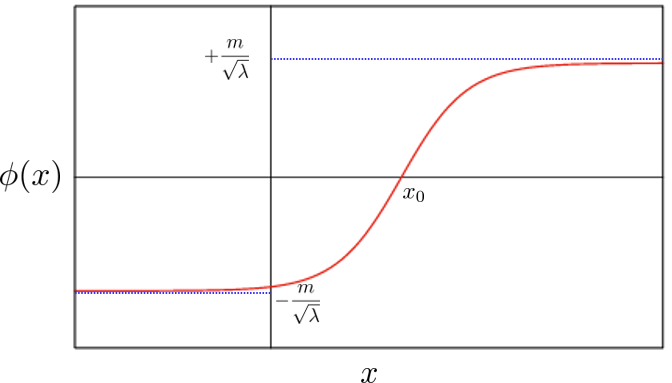
\includegraphics[width=10cm]{figure/kink_phi.png}
    \caption{kink解($\phi(x)$)}
    \label{kink_phi}
\end{figure}
また,kink解のエネルギー密度は
\begin{align}
    \epsilon(x) & =\frac{1}{2}(\phi')^2+U(\phi)=2U(\phi),\quad \text{using (\ref{eq:2.22})} \\
                & =(m^4/2\lambda)\mathrm{sech^4}\left[m(x-x_0)/\sqrt{2}\right]
\end{align}
となり,これをグラフにプロットすれば図\ref{kink_energy}のようになり確かにlocalizeしていることがわかる.

また,kinkのエネルギー密度の合計はclassical kinkmass $M_{\mathrm{cl}}$と呼ばれ
\begin{align}
    M_{\mathrm{cl}}=\int_{-\infty}^{\infty} \mathrm{d}x \epsilon(x)=\dfrac{2\sqrt{2}}{3}\frac{m^3}{\lambda}
\end{align}
で与えられ,有限の値を取る.

以上のことから正のkinkや負のanti-kinkはまさに真のSolitary waveであるといえる.しかしながらkinkやanti-kinkはどちらもSolitonではない.
\begin{figure}[H]
    \centering
    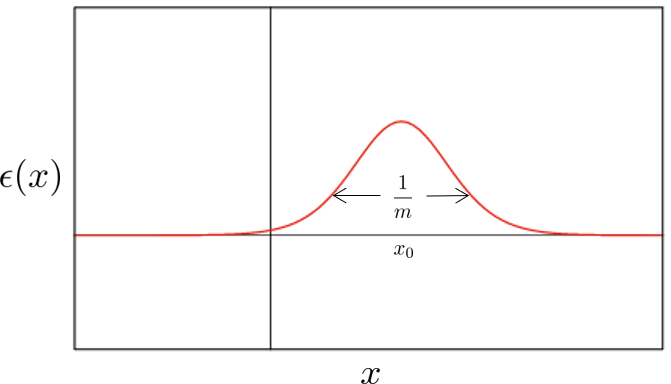
\includegraphics[width=10cm]{figure/kink_energy.png}
    \caption{kink解($\epsilon(x)$)}
    \label{kink_energy}
\end{figure}

\subsubsection{Lorentz-transform to the static solution}
いま求めたkink解はローレンツ不変な量であることがわかっており,静的な解をローレンツ変換することによって動くkink解を得ることができる.したがって式(\ref{eq:2.28})を速度$1>u>-1$で動く系でローレンツ変換をすれば
\begin{align}
    \phi_{u}(x, t)=\frac{m}{\sqrt{\lambda}} \tanh \left[\frac{m}{\sqrt{2}}\left(\frac{\left(x-x_{0}\right)-u t}{\sqrt{1-u^{2}}}\right)\right]\label{eq:2.32}
\end{align}
となる.(式(\ref{eq:2.25})に代入すればこれが解になっていることも確かめられる.)またこの動的なkink解の幅は$\sqrt{1-u^2}/m$となっており,ローレンツ収縮が起きていることも見て取れる.実際,時間依存するkink解(\ref{eq:2.32})のエネルギーを計算すると
\begin{align}
    E\left[\phi_{u}\right]= & \int_{-x}^{x} \mathrm{d} x\left[\frac{1}{2}\left(\dot{\phi}_{u}\right)^{2}+\frac{1}{2}\left(\phi_{u}^{'}\right)^{2}+U\left(\phi_{u}\right)\right]\nonumber                           \\
    =                       & \int_{-x}^{x} \mathrm{d} x\left[\left(\frac{m^{4}}{4 \lambda} \frac{u^{2}}{1-u^{2}}+\frac{m^{4}}{4 \lambda} \frac{1}{1-u^{2}}+\frac{m^{4}}{4 \lambda}\right)\right.\nonumber         \\
                            & \qquad\ \ \ \ \ \ \ \ \ \ \ \  \times\left.\operatorname{sech}^{4}\left(\frac{m}{\sqrt{2}} \frac{x-x_{0}-u t}{\sqrt{1-u^{2}}}\right)\right]\nonumber                                 \\
                            & =\int_{-\infty}^{\infty} \mathrm{d} x \frac{m^{4}}{2 \lambda\left(1-u^{2}\right)} \operatorname{sech}^{4}\left(\frac{m}{\sqrt{2}} \frac{x-x_{0}-u t}{\sqrt{1-u^{2}}}\right)\nonumber \\
                            & =\frac{2 \sqrt{2}}{3} \frac{m^{3}}{\lambda} \frac{1}{\sqrt{1-u^{2}}}\nonumber                                                                                                        \\
                            & =\frac{M_{\mathrm{cl}}}{\sqrt{1-u^{2}}}
\end{align}
となり,静的な$M_{\mathrm{cl}}$に対してローレンツ収縮が起きていることがわかる.

\subsubsection{Case of $U(\phi)$ has three degenerate minima}
$U(\phi)$が3つの最小値をもつ縮退した例として以下のポテンシャルを考える.
\begin{align*}
    U(\phi)=\frac{1}{2} \phi^{2}\left(\phi^{2}-1\right)^{2}
\end{align*}
この最小値は$\phi=0,\pm1$で縮退しており境界条件は
\begin{align*}
    \phi=[-1,0],[0,1],[1,0] \text { and }[0,-1] \quad \text { at } x=[-\infty, \infty]
\end{align*}
のように設定できる.また具体的な計算は行わないが式(\ref{eq:2.17})にこれを代入し解いた結果は
\begin{align}
    \phi=\pm\left(1+e^{\pm 2 x}\right)^{-\frac{1}{2}}
\end{align}
となる.この解もlocalizeしたエネルギー密度をもち,全エネルギーは有限となる.

\subsection{Static solutions to system of coupled scalar fields}
先の議論では1つの場$\phi$に対する解の考察であったが,2つ以上の場がcoupleしてできる静的な解についても考察する.以下のようなラグランジアン密度を考える.
\begin{align}
    \mathscr{L}(\mathrm{x}, \mathrm{t})=\sum_{\mathrm{i}=1}^{\mathrm{N}} \frac{1}{2}\left(\left(\frac{\partial \phi_{\mathrm{i}}}{\partial \mathrm{t}}\right)^{2}-\left(\frac{\partial \phi_{\mathrm{i}}}{\partial \mathrm{t}}\right)^{2}\right)-\mathrm{U}\left(\left\{\phi_{\mathrm{i}}\right\}\right)
\end{align}
このとき場の方程式は
\begin{align}
    \square \phi_{i}=-\frac{\partial U}{\partial \phi_{i}} ; \quad i=1, \ldots, N
\end{align}
となり,静的な場合時間の項を削除して
\begin{align}
    \phi''=\frac{\partial U}{\partial\phi_i}\label{eq:2.37}
\end{align}
となる.これもよく見れば前回と同様に$x\rightarrow t$, $\phi_i\rightarrow x_i$とすればポテンシャル$[-U(\phi)]$のanalogue粒子の描像(有限作用,ゼロエネルギーの軌道)と捉え直すことが可能となる.しかし1つの場の場合と異なる点が以下のように2点ある.
\begin{description}
    \item[(i)] 1つの場の場合は$U(\phi)$の最小値が1つのとき,$t\rightarrow -\infty$で運動エネルギーが常に正となり二度とスタート地点に戻ることはなく,Solitary waveが存在し得なかった.しかし複数の場がある場合は$N$次元$\phi_i$空間において同様に運動エネルギーが正のままだが,閉曲線に沿って再びスタート地点に戻る可能性がある.
    \item[(ii)] 複数の場があるがゆえに式(\ref{eq:2.37})において具体的な$\phi_i$の関数を定めるための積分が容易にできない.複数の場においても積分ができるのは力学との対応関係から,ポテンシャルが中心力ポテンシャルの形になるもの(極座標系でかくと簡単になる),つまり本文においては$\phi_i$の回転のもとで不変性が保てるものである.(内部対称性(internal symmetry))
\end{description}

\subsubsection{How to solve}
実際に式(\ref{eq:2.37})を解くことを試みる.まず我々がすべきことは$N$次元$\phi_i$空間におけるanalogue粒子の軌道をみつけることである.というのも$\phi_i$空間における軌道が分かればその軌道に沿って積分を行えば良いからである.

例として2つの場$\phi_1, \phi_2$が作る$U(\phi_1, \phi_2)$について考える.この場合analogue粒子は$\phi_1,\phi_2$平面上を$U(\phi_1,\phi_2)$に沿って移動する.$U(\phi_1,\phi_2)$が点Pおよび点Qの2点で縮退した最小値をとるとすれば,その間をポテンシャルに沿って移動することは前回同様である.その軌道を
\begin{align}
    g(\phi_1,\phi_2)=0
\end{align}
とすれば
\begin{align}
    \frac{\mathrm{d}g(\phi_1,\phi_2)}{\mathrm{d}x}=0\nonumber                                                                                                            \\
    \Rightarrow \frac{\partial g}{\partial \phi_1}\frac{\mathrm{d}\phi_1}{\mathrm{d}x}+\frac{\partial g}{\partial \phi_2}\frac{\mathrm{d}\phi_2}{\mathrm{d}x}=0\nonumber \\
    \Rightarrow \frac{\partial g}{\partial \phi_1}\phi_1'+\frac{\partial g}{\partial \phi_2}\phi_2'=0\nonumber                                                           \\
    \Rightarrow \left(\frac{\partial g}{\partial \phi_{1}}\right)^{2}\left(\phi_{1}^{'}\right)^{2}=\left(\frac{\partial g}{\partial \phi_{2}}\right)^{2}\left(\phi_{2}^{'}\right)^{2}\label{eq:2.39}
\end{align}
となる.また,式(\ref{eq:2.37})を両辺積分して
\begin{align}
    \frac{1}{2}\left(\phi_{i}^{'}\right)^{2}=\int \frac{\partial U\left(\phi_{1}, \phi_{2}\right)}{\partial \phi_{i}} \mathrm{d} \phi_{i}+A_{i}\quad; \quad i=1,2\label{eq:2.40}
\end{align}
を得る.そして式(\ref{eq:2.39})を式(\ref{eq:2.40})に代入すれば
\begin{align}
    \left(\frac{\partial g}{\partial \phi_{1}}\right)^{2}\left(\int \frac{\partial U\left(\phi_{1}, \phi_{2}\right)}{\partial \phi_{1}} \mathrm{d} \phi_{1}+A_{1}\right)=\left(\frac{\partial g}{\partial \phi_{2}}\right)^{2}\left(\int \frac{\partial U\left(\phi_{1}, \phi_{2}\right)}{\partial \phi_{2}} \partial \phi_{2}+A_{2}\right)\label{eq:2.41}
\end{align}
として$g(\phi_1,\phi_2)$と$U(\phi_1,\phi_2)$が直接結びついた軌道の方程式を得る.ここに具体的な軌道$g(\phi_1,\phi_2)$とポテンシャル$U(\phi_1,\phi_2)$を代入していくことで$\phi_1,\phi_2$についてこの方程式を解くことができる.まず軌道としては図\ref{orbit1}に示すように以下の3パターンが考えうる.ここでType Cに関しては$U=0$になることによって運動エネルギーが常に正であるという知見から一見すると起こり得ないため,(引き返すためには点Rで一度運動エネルギーが0になる必要がある.)\footnote{しかし8章で紹介するが静的なSolitary waveではなく,"charge"された解の場合はこのようなことが起こりうる.}以下ではType A及びType Bについて見ていく.
\begin{description}
    \item[Type A] $U(\phi_1,\phi_2)$の最小値の1つであるPまたはQのどちらかからスタートし,再びおなじスタート地点に戻る閉曲線軌道.
    \item[Type B] $U(\phi_1,\phi_2)$の最小値の1つであるPかQのどちらかからスタートし,スタート地点とは異なるPかQの地点にゴールする軌道.
    \item[Type C] $U(\phi_1,\phi_2)$の最小値の1つであるPまたはQのどちらかからスタートし,任意のPへ引き返す経路.
\end{description}

\begin{figure}[H]
    \centering
    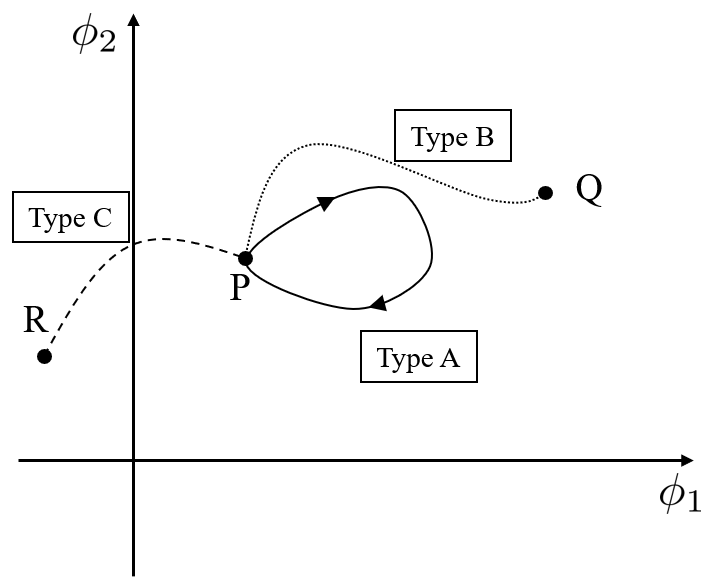
\includegraphics[width=7cm]{figure/orbit1.png}
    \caption{軌道}
    \label{orbit1}
\end{figure}

例としてポテンシャルを
\begin{align}
     & U\left(\phi_{1}, \phi_{2}\right)=\frac{1}{4}\left(\phi^{2}-1\right)^{2}+\frac{1}{2} m^{2}\left(\phi_{2}\right)^{2}+\frac{1}{4} \lambda\left(\phi_{2}\right)^{4}+\frac{1}{2} d \phi_{2}^{2}\left(\phi_{1}^{2}-1\right)\label{eq:2.42} \\
     & \qquad \ \ \ \ \ \ \ \ \ \ \ \ \ \ \ \ \ \ \ \ \ \ \ \ \ \ \ \ \ \ \ \ \ \ \ \ \ \ \ \ \ \ \ \ \ \ \ \ \ \ \ \ \ \ \ \ \ \ \ \ \ \ (\lambda, d, m^2 >0)\nonumber
\end{align}
とする.これは図\ref{phi4_model}のように$\{\phi_1,\phi_2\}=\{1,0\},\{-1,0\}$の2点で最小値をとる模型となる.(ただし$\lambda \leq (d-m^2)^2$.)

\begin{figure}[H]
    \centering
    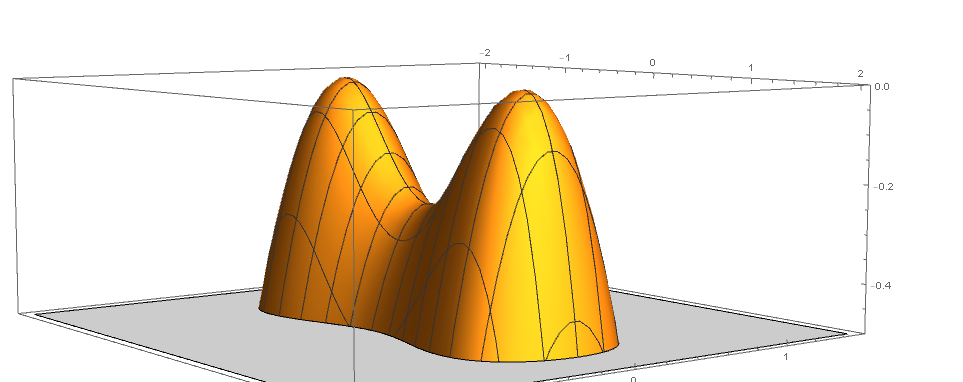
\includegraphics[width=8cm]{figure/phi4_model.png}
    \caption{}
    \label{phi4_model}
\end{figure}

いまType Bの軌道を取る場合について任意定数$\alpha,n$を用いて多項式展開の形で
\begin{align}
    g\left(\phi_{1}, \phi_{2}\right)=\left(\phi_{2}\right)^{n}+\alpha\left(\left(\phi_{1}\right)^{2}-1\right)=0\quad ; \quad (n=1,2)\label{eq:2.43}
\end{align}
とする.軌道が$\{\phi_1,\phi_2\}=\{-1,0\}$からスタートするとして式(\ref{eq:2.43})を式(\ref{eq:2.41})に代入すれば
\begin{align}
     & \left(2 \alpha \phi_{1}\right)^{2}\left(\int_{-1}^{\phi_{1}} \mathrm{d} \tilde{\phi}_{1}\left(\tilde{\phi}_{1}^{3}-\tilde{\phi}_{1}+\mathrm{d} \tilde{\phi}_{2}^{2} \tilde{\phi}_{1}\right)\right)\nonumber                                                \\
     & \qquad\ \ \ \ \ \ \ \ =\left(n \phi_{2}^{n-1}\right)^{2}\left(\int_{0}^{\phi_{2}} \mathrm{d} \phi_{2}\left(m^{2} \tilde{\phi}_{2}+\lambda \tilde{\phi}_{2}^{3}+\mathrm{d} \tilde{\phi}_{2}\left(\tilde{\phi}_{1}^{2}-1\right)\right)\right)\label{eq:2.44}
\end{align}
となる.(なお,境界条件から式(\ref{eq:2.40})において$A_i=0$としている.)またこの積分を実行した上で式(\ref{eq:2.43})の関係から$\phi_1$を消去すれば
\begin{align}
     & 4 \alpha^{2}\left(1-\frac{\phi_{2}^{n}}{\alpha}\right)\left(\frac{\phi_{2}^{2 n}}{4 \alpha^{2}}-\frac{n d}{2 \alpha(n+2)} \phi_{2}^{n+2}\right)\nonumber           \\
     & \qquad\ \ \ \ \ \ \ \ =\frac{1}{2} m^{2} n^{2} \phi_{2}^{2 n}+\frac{1}{4} \lambda n^{2} \phi_{2}^{2 n+2}-\frac{d n^{2} \phi_{2}^{3 n}}{\alpha(n+2)}\label{eq:2.45}
\end{align}

ここで式(\ref{eq:2.45})の右辺を展開して左辺との係数比較をすることで定数を決定する.
\begin{description}
    \item[(i)] $n=2$の場合\\
          \begin{align}
              \alpha=\frac{\left(1-2 m^{2}\right)}{d}, \quad \lambda=\frac{d\left(d-2 m^{2}\right)}{1-2 m^{2}}
          \end{align}
          となり,式(\ref{eq:2.44})に代入すれば軌道として
          \begin{align*}
              \phi_2^2=\left[(1-2m^2)/d\right](1-\phi_1^2)
          \end{align*}
          の関係を得る.そしてこれを場の方程式(\ref{eq:2.37})に代入し,積分を実行すれば
          \begin{align}
               & \phi_1''=\phi_1^3-\phi_1+d\phi_2^2\phi_1=2m^2(\phi_1^3-\phi_1) \\
               & \Rightarrow
              \begin{cases}
                  \phi_{1}(x)=\tanh \left[m\left(x-x_{0}\right)\right] \\
                  \phi_{2}(x)=\pm\left[\left(1-2 m^{2}\right) / d\right]^{1 / 2} \operatorname{sech}\left[m\left(x-x_{0}\right)\right]
              \end{cases}\label{eq:2.48}
          \end{align}
          としてSolitary waveの解を得ることができる.
    \item[(ii)] $n=1$の場合\\
          \begin{align}
              m^{2}=2, \quad \lambda=\frac{8}{3} d, \quad \alpha^{2}=(d-3)/2
          \end{align}
          となり,先の議論と同様に式(\ref{eq:2.44})に代入すれば軌道として
          \begin{align*}
              \phi_{2}=[(d-3) / 2 d]^{1 / 2}\left(1-\phi_{1}^{2}\right)
          \end{align*}
          の関係を得て,場の方程式(\ref{eq:2.37})に代入すれば
          \begin{align}
              \phi_{2}^{''} & =m^{2} \phi_{2}+\lambda \phi_{2}^{3}+d \phi_{2}\left(\phi_{1}^{2}-1\right)\nonumber \\
                            & =2 \phi_{2}-d[2 d /(d-3)]^{1 / 2} \phi_{2}^{2}+\frac{8}{3} d \phi_{2}^{3}
          \end{align}
          となり,定数$a,b,c$を用いて解きやすい形にして積分を実行すれば
          \begin{align}
              \phi_{2}^{''}=a \phi_{2}-\frac{3}{2} b \phi_{2}^{2}+2 c \phi_{2}^{3} \\
              \Rightarrow
              \begin{cases}
                  \phi_{2}(x)=\frac{2 a}{\left(b^{2}-4 a c\right)^{1 / 2} \cosh (\sqrt{a} x)+b} \\
                  \phi_{1}^{2}(x)=1-[2 d /(d-3)]^{1 / 2} \phi_{2}(x)
              \end{cases}\label{eq:2.52}
          \end{align}
          を得る.
\end{description}
以上の手順で式(\ref{eq:2.48})及び式(\ref{eq:2.52})でSolitary wave解を得て,概形としてはどちらも同じで図\ref{2-coupled-phi_typeB}のようになる.
\begin{figure}[H]
    \centering
    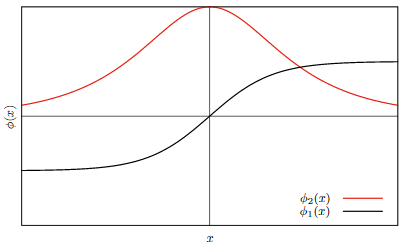
\includegraphics[width=10cm]{figure/2-coupled-phi_typeB.png}
    \caption{}
    \label{2-coupled-phi_typeB}
\end{figure}

また,Type Aのような同じスタート地点に戻る閉曲線軌道のものに関しても
\begin{align}
    g\left(\phi_{1}, \phi_{2}\right)=\phi_{2}^{2}-\beta\left(\phi_{1}+1\right)\left(\alpha-\phi_{1}\right)=0
\end{align}
と置いて式(\ref{eq:2.41})から同様の手順を踏むことで
\begin{align}
     & \alpha                    =\frac{1+4 m^{2}}{3}, \quad \beta=\frac{2-4 m^{2}}{1+4 m^{2}}, \quad d=\frac{3+12 m^{2}}{4+4 m^{2}},\quad \lambda=\frac{\left(5-4 m^{2}\right)\left(1+4 m^{2}\right)}{\left(8+8 m^{2}\right)\left(1-2 m^{2}\right)}, \\
     & \phi_{1}^{\prime \prime}= 4 m^{2}\left(1+\phi_{1}\right)-\left(\frac{8\left(1+m^{2}\right)^{2}-9}{2\left(1+m^{2}\right)}\right)\left(1+\phi_{1}^{2}\right)^{2}\nonumber                                                                        \\
     & \qquad\ \ \ \ \ \ \ \ \ \ \ \ \ \ \ \ \ \ \ \ \ \ \ \ \ \ \ \ \ \ \ \ \ \ \ \ +\left(\frac{8 m^{2}-1}{2\left(1 + m^{2}\right)}\right)\left(1+\phi_{1}\right)^{3}                                                                               \\
     & \Rightarrow \phi_{1}(x)=\frac{2 a}{\left(b^{2}-4 a c\right)^{1 / 2} \cosh (\sqrt{a} x)+b}-1
\end{align}
のように各計算過程が定まり,その概形は図\ref{2-coupled-phi_typeA}のようになる.
\begin{figure}[H]
    \centering
    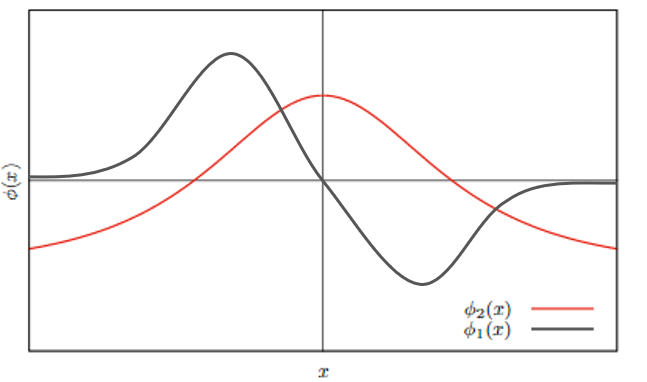
\includegraphics[width=10cm]{figure/2-coupled-phi_typeA.png}
    \caption{}
    \label{2-coupled-phi_typeA}
\end{figure}
以上で式(\ref{eq:2.48})のような複合場が作るポテンシャルにおいて,それそれの場の厳密解を求めることができた.以下にその手順をまとめておく.
\begin{screen}
    \begin{description}
        \item[(i)] analogue粒子が描く軌道を設定し,その方程式をたてる.
        \item[(ii)] 軌道とポテンシャルの間の関係を導き,(i)で定めた方程式を代入して出来上がる恒等式の係数比較をすることで各パラメータを決定する.
        \item[(iii)] 軌道の方程式に(ii)で定まった各パラメータを代入し,積分方程式を解くことで厳密解を得る.
    \end{description}
\end{screen}


\section{Topological indices}
本セクションでは時間変化のなかで保存するトポロジカルな指標(Topological indices)とはどのようなものかを具体的に見ていく.なお,Topological indicesは量子場の理論における粒子状態に対する量子数として重要な役割を果たす.

複合場ではなく,1つの場$\phi$が作る(1+1)次元系において話を進める.ポテンシャルは式(\ref{eq:2.24})の
\begin{align*}
    \mathscr{L}(x, t)=\frac{1}{2}\left(\frac{\partial \phi}{\partial t}\right)^{2}-\frac{1}{2}\left(\frac{\partial \phi}{\partial x}\right)^{2}-U(\phi)\nonumber \\
    U(\phi)=\frac{1}{4}\lambda(\phi^2-m^2/\lambda)^2
\end{align*}
の状況で考える.このSolitary waveを特徴づけるのは$\phi=\pm/\sqrt{\lambda}$で$U(\phi)=0$となる条件から以下の4つのtopological indicesとなる.
\begin{align}
     & \left(\phi(x=-\infty),\phi(x=+\infty)\right)=\nonumber                                                                                                                \\
     & (-m/\sqrt{\lambda},m/\sqrt{\lambda}),\quad (m/\sqrt{\lambda},-m/\sqrt{\lambda}),\quad (-m/\sqrt{\lambda},-m/\sqrt{\lambda}),\quad (m/\sqrt{\lambda},m/\sqrt{\lambda})
\end{align}
これらは左から順にkink解,anti-kink解,定数解$\phi(x)=\mp(m/\sqrt{\lambda})$の4つである.例えば左からkink解,右からanti-kink解が衝突するような状況を考えたときに,衝突後どのような様子を描くかは用意にはわからないが,衝突前も衝突後も$\left(\phi(x=-\infty),\phi(x=+\infty)\right)=(-m/\sqrt{\lambda},-m/\sqrt{\lambda})$というtopologicalセクターに属するということは常にわかる.

\subsection{Topological charge}
Topological indicesに関連してTopological chargeという量がしばしば用いられ,本ポテンシャルの場合以下で定義される.
\begin{align}
    Q=\frac{\sqrt{\lambda}}{m}[\phi(x=\infty)-\phi(x=-\infty)]
\end{align}
また,これに対する保存カレントとして
\begin{align}
    k^{\mu}=\frac{\sqrt{\lambda}}{m} \varepsilon^{\mu \nu} \partial_{\nu} \phi;\quad \mu,\nu=0,1;\quad g_{\mu \nu}=
    \begin{pmatrix}
        1 & 0  \\
        0 & -1
    \end{pmatrix}
\end{align}
が挙がる.($\varepsilon^{\mu\nu}$は反対称テンソル.)これらを用いればきれいな形で
\begin{align}
    \partial_{\mu} k^{\mu}=0 \quad \text { and } \quad Q=\int_{-\infty}^{\infty} \mathrm{d} x k_{0}
\end{align}
を得る.まさにTopological charge $Q$は$(\sqrt{\lambda}/m)\phi(\infty)$と$(\sqrt{\lambda}/m)\phi(\infty)$の値の差であり,$Q=0$または$Q\neq 0$のどちらかを取る.先に上げた4つのtopological indicesのうち$Q\neq0$となるのは$(-m/\sqrt{\lambda},m/\sqrt{\lambda}),(m/\sqrt{\lambda},-m/\sqrt{\lambda})$の2つのkink及びanti-kinkでtopologicalな解と呼ぶ.実際,このtopological chargeが一種の境界条件となっており,$Q\neq0$でtopologicalであれば非自明な静的Solitary wave解を得ることができるということを意味する.これは次元が増えようとも,空間変換,ゲージ変換をしようとも具体的な解の計算前にいつでもモデルのtopologyを調べることができるとても強力なツールとなる.

\section{Soliton of the sine-Gordon system}
章の最後にSoliton解として有名なsine-Gordonの解を見ていく.このラグランジアン密度は
\begin{align}
    \mathscr{L}(x, t)=\frac{1}{2}\left(\partial_{\mu} \phi\right)\left(\partial^{\mu} \phi\right)+\left(m^{4} / \lambda\right)\{\cos [(\sqrt{\lambda} / m) \phi]-1\}\label{eq:2.61}
\end{align}
で与えられる.またこのラグランジアンは相転移の伝播,Josephson line中での磁束の伝播や荷電粒子の2次元モデルなど様々な模型に使われている.また式(\ref{eq:2.61})を$\lambda$についてべき展開した
\begin{align}
    \mathscr{L}(x, t)=\frac{1}{2}\left(\partial_{\mu} \phi\right)\left(\partial^{\mu} \phi\right)-\frac{1}{2} m^{2} \phi^{2}+\frac{\lambda}{4 !} \phi^{4}-\frac{\lambda^{2} \phi^{6}}{m^{2} 6 !}+\ldots
\end{align}
もKlein-Gordonの系を作るとして非常に有名である.

そして,話を式(\ref{eq:2.61})に戻せば,このラグランジアンが作る方程式は
\begin{align*}
    \square \phi+\left(m^{3} / \sqrt{\lambda}\right) \sin [(\sqrt{\lambda} / m) \phi]=0 .
\end{align*}
となる.式を簡単にするために
\begin{align}
    \bar{x}=m x, \quad \bar{t}=m t \quad \text { and } \quad \bar{\phi}=(\sqrt{\lambda} / m) \phi .
\end{align}
と変数変換すればラグランジアン密度及び運動方程式は
\begin{align}
    \bar{\mathscr{L}}(\bar{x}, \bar{t})=\left(m^{4} / \lambda\right)\left[\frac{1}{2}\left(\bar{\partial}_{\mu} \bar{\phi}\right)\left(\bar{\partial}^{\mu} \bar{\phi}\right)+(\cos \bar{\phi}-1)\right]\label{eq:2.64} \\
    \frac{\partial^{2} \bar{\phi}}{\partial \bar{t}^{2}}-\frac{\partial^{2} \bar{\phi}}{\partial \bar{x}^{2}}+\sin \bar{\phi}(\bar{x}, \bar{t})=0\label{eq:2.65}
\end{align}
となる.そしてエネルギー積分は
\begin{align}
    E=\frac{m^{3}}{\lambda} \int \mathrm{d} \bar{x}\left[\frac{1}{2}\left(\frac{\partial \bar{\phi}}{\partial \bar{t}}\right)^{2}+\frac{1}{2}\left(\frac{\partial \bar{\phi}}{\partial \bar{x}}\right)^{2}+(1-\cos \bar{\phi})\right]\label{eq:2.66}
\end{align}
となる.また,このラグランジアンと場の方程式は対称性があることがわかっており
\begin{align}
     & \bar{\phi}(\bar{x}, \bar{t}) \rightarrow-\bar{\phi}(\bar{x}, \bar{t})                                             \\
     & \bar{\phi}(\bar{x}, \bar{t}) \rightarrow \bar{\phi}(\bar{x}, \bar{t})+2 N \pi ; \quad N=\ldots-2,-1,0,1,2, \ldots
\end{align}
の関係性をもっている.この対称性を用いてればエネルギー$E$は最小値である
\begin{align}
    U(\bar{\phi})=1-\cos \bar{\phi}\quad \text{which are} \quad \bar{\phi}(\bar{x}, \bar{t})=2 N \pi
\end{align}
で消える.つまりこのラグランジアンのTopologicalセクターは$\left(\phi(x=-\infty),\phi(x=+\infty)\right)=(N_1,N_2)=(-2N_1\pi, 2N_2\pi)$であることが前セクションでの議論によってわかる.そしてTopological chargeを計算することによって静的なのか,時間依存なのかを知ることができる.いま仮に$\bar{\phi}$のモジュールである$2\pi$が物理的に意味があるとすればTopological chargeは
\begin{align}
    Q \equiv N_{1}-N_{2}=\frac{1}{2 \pi} \int_{-\infty}^{\infty} \mathrm{d} \bar{x} \frac{\partial \bar{\phi}}{\partial \bar{x}}
\end{align}
で定義される.

\subsection{Static localised solution}
まず静的で局在化する解について考える.この場合,$Q=\pm 1$である必要があり,式(\ref{eq:2.23})で導いた関係を用いれば
\begin{align}
    \bar{x}-\bar{x}_{0}=\pm \int_{\bar{\phi}\left(\bar{x}_{0}\right)}^{\bar{\phi}(\bar{x})} \frac{\mathrm{d} \phi}{\sqrt{2 U(\phi)}}=\pm \int_{\bar{\phi}(\bar{x}_{0})}^{\phi(\bar{x})} \frac{\mathrm{d} \phi}{2 \sin (\phi / 2)}
\end{align}
\begin{subequations}
    \begin{align}
        \Rightarrow \bar{\phi}(x)=4 \tan ^{-1}\left[\exp \left(\bar{x}-\bar{x}_{0}\right)\right] \equiv \phi_{\mathrm{sol}}\left(\bar{x}-\bar{x}_{0}\right)\label{eq:2.72a} \\
        \Rightarrow \bar{\phi}(x)=-4 \tan ^{-1}\left[\exp \left(\bar{x}-\bar{x}_{0}\right)\right] \equiv \bar{\phi}_{\text {antisol }}\left(\bar{x}-\bar{x}_{0}\right)=-\bar{\phi}_{\text {sol}}\label{eq:2.72b}
    \end{align}
\end{subequations}
の2つの解を得ることができる.ここで,式(\ref{eq:2.72a})は図\ref{eq2-72_fig}のように$\bar{\phi}=0$から$\bar{\phi}=2\pi$または$2\pi$から$4\pi$,$4\pi$から$6\pi$というように変化し,$Q=1$となる.そしてこれはSolitonと呼ばれる.
\begin{figure}[H]
    \centering
    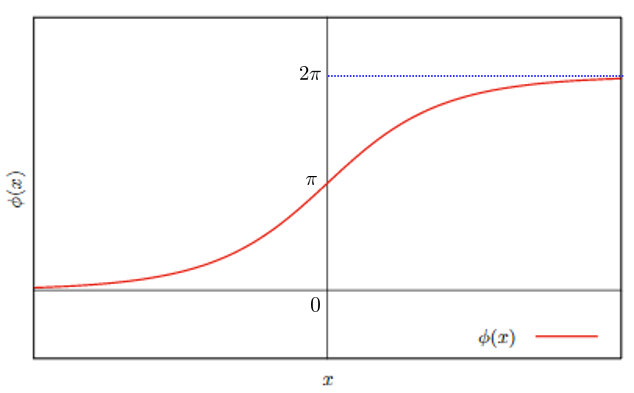
\includegraphics[width=10cm]{figure/eq2-72.png}
    \caption{}
    \label{eq2-72_fig}
\end{figure}
一方で式(\ref{eq:2.72b})は$Q=-1$でAnti-solitonと呼ばれている.また,どちらの解も式(\ref{eq:2.66})に代入することでエネルギー$M_\mathrm{s}=8m^3/\lambda$を持つこともわかる.さらにもし仮にこのSoliton解を動かしたければ以前行ったのと同様にローレンツ変換を行い,$(\bar{x}-\bar{x}_0)$を$\left[\left(\bar{x}-\bar{x}_{0}-u \bar{t}\right) / \sqrt{1-u^{2}}\right]$とように変換すれば良い.

\subsection{Behavior of Soliton solution}
式(\ref{eq:2.72a})及び式(\ref{eq:2.72b})のSoliton解は一見するとkink解と同様に思える.しかしながら,しっかりと式(\ref{eq:2.9})(\ref{eq:2.10})のSolitonとしての強い要請を満たしているのである.そこでいくつかのSolitonを衝突させた場合の振る舞いを見ていく.そこでSoliton解とAnti-Soliton解を重ね合わせた,同じく式(\ref{eq:2.65})の方程式を満たす以下のような解を考える.
\begin{align}
    \bar{\phi}_{\mathrm{SA}}(\bar{x}, t)=4 \tan ^{-1}\left(\frac{\sinh \left(u \bar{t} / \sqrt{1-u^{2}}\right)}{u \cosh \left(\bar{x} / \sqrt{1-u^{2}}\right)}\right)
\end{align}
これがSoliton解とAnti-solitonを重ね合わせて形を保つということは以下のように容易に示せる.
\begin{align}
    \bar{\phi}_{\mathrm{SA}}(\bar{x}, \bar{t}) \underset{\bar{t} \rightarrow-\infty}{\longrightarrow} 4 \tan ^{-1}\left[\exp \left(\frac{\bar{x}+u(\bar{t}+\Delta / 2)}{\sqrt{1-u^{2}}}\right)\right]\nonumber                                                                                  \\
    -4 \tan ^{-1}\left[\exp \left(\frac{\bar{x}-u(\bar{t}+\Delta / 2)}{\sqrt{1-u^{2}}}\right)\right]\nonumber                                                                                                                                                                                   \\
    =\bar{\phi}_{\mathrm{sol}}\left(\frac{\bar{x}+u(\bar{t}+\Delta / 2)}{\sqrt{1-u^{2}}}\right)+\bar{\phi}_{\text {antisol }}\left(\frac{\bar{x}-u(\bar{t}+\Delta / 2)}{\sqrt{1-u^{2}}}\right)                                                                                                  \\
    \bar{\phi}_{\mathrm{SA}}(\bar{x}, \bar{t}) \underset{\bar{t} \rightarrow-\infty}{\longrightarrow} \bar{\phi}_{\mathrm{sol}}\left(\frac{\bar{x}+u(\bar{t}-\Delta / 2)}{\sqrt{1-u^{2}}}\right)+\bar{\phi}_{\text {antisol }}\left(\frac{\bar{x}-u(\bar{t}-\Delta / 2)}{\sqrt{1-u^{2}}}\right) \\
    \Delta \equiv\left(\left(1-u^{2}\right) / u\right) \ln u
\end{align}
なお,描像については別ファイルのgifを参照.

\appendix
\chapter{How to define energy density}
エネルギー運動量テンソルは
\begin{align*}
    T^{\mu \nu}=\frac{\partial \mathcal{L}}{\partial\left(\partial_{\mu} \phi\right)} \partial^{\nu} \phi-\eta^{\mu \nu} \mathcal{L}
\end{align*}
で定義され,エネルギー密度$\epsilon$を知りたければ$T^{00}$を計算すればよい.ラグランジアン密度が
\begin{align*}
    \mathcal{L}(t,x)=\frac{1}{2}\left(\partial_{t} \phi\right)^{2}-\frac{1}{2}\left(\partial_{x} \phi\right)^{2}-U
\end{align*}
で記述されるとすれば
\begin{align*}
    T^{00}= & \frac{\partial \mathcal{L}}{\partial\left(\partial_{0} \phi\right)} \partial^{0} \phi-\eta^{00} \mathcal{L}                                                                                        \\
    =       & \left(\partial_{t} \phi\right) \frac{\partial}{\partial\left(\partial_{t} \phi\right)}\left\{\frac{1}{2}\left(\partial_{t} \phi\right)^{2}-\frac{1}{2}\left(\partial_{x} \phi\right)^{2}-U\right\} \\
            & -\left\{\frac{1}{2}\left(\partial_{t} \phi\right)^{2}-\frac{1}{2}\left(\partial_{x} \phi\right)^{2}-U\right\}                                                                                      \\
    =       & \left(\partial_{t} \phi\right)^{2}-\frac{1}{2}\left(\partial_{t} \phi\right)^{2}+\frac{1}{2}\left(\partial_{x} \phi\right)^{2}+U                                                                   \\
    =       & \frac{1}{2}\left(\partial_{t} \phi\right)^{2}+\frac{1}{2}\left(\partial_{x} \phi\right)^{2}+U
\end{align*}
となり,エネルギー密度は
\begin{align*}
    \mathcal{E}(t, x)=\frac{1}{2}\left(\partial_{t} \phi\right)^{2}+\frac{1}{2}\left(\partial_{x} \phi\right)^{2}+U
\end{align*}
として定めることができる.そして系全体のエネルギーはこれを全空間で積分すればよく,
\begin{align*}
    E[\phi]=\int_{-\infty}^{+\infty} \mathrm{d} x \mathcal{E}(t, x)
\end{align*}
で与えられる.




\end{document}
